\section{H-bro test}\label{sec:bilag_hbrotest}
For at p�vise, at H-broen fungerer til at �ge Scalextricbilens bremseevne, er der foretaget en r�kke fors�g. Som beskrevet i sektion \ref{sec:hbro}, er form�let med H-broen at bremse bilen. Hvor stor en kraft motoren skifter retning med, kan vha. microcontrolleren justeres alt efter hvilke v�rdier der sendes til bilen. Der sendes en hexadecimal v�rdi fra 0x00-0xFF til bilen, hvor 0x00 er ingen v�rdi og 0xFF er max bagud/forud-rettet kraft. 0x00 har ingen effekt p� bilen og den vil forts�tte up�virket. Des h�jere v�rdien s�ttes til, des st�rre kraft bremses bilen med. P� Figur \ref{fig:hbrotest} kan der ses de 3 bremsel�ngder med henholdsvis a0, kortslutning og fri l�b.

\begin{figure}[htb]
\center
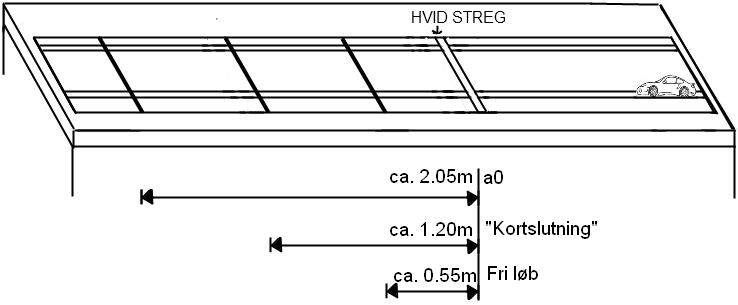
\includegraphics[scale=0.5]{hbrotest.png}
\caption{H-bro test}
\label{fig:hbrotest}
\end{figure}

Som der ses p� figuren, er der markeret en hvid streg p� skinnen, som optosensoren opfanger. N�r bilen passere denne streg t�ndes H-broen med den v�rdi der nu er sendt til den. Som tidligere n�vnt skifter motoren retning og hastigheden daler hurtigt. Efter kort tid vil bilen i et kort �jeblik st� stille og bakke. Netop dette �jeblik registreres med m�leb�nd og �jet. Udfra Figur \ref{fig:hbrotest} ses der at jo st�rre Hex V�rdi der sendes, jo kortere bremsel�ngde har bilen. Konklusionen p� dette fors�g er, at H-broen virker ubeklageligt. 